\section{Resultados obtenidos}
\label{sec:results}

Los resultados de precisión para todos los modelos y \textit{datasets} utilizados se muestran en la tabla \hyperref[tab:acc]{6.1}. Observamos que los modelos \emph{Bag of Words} (BoW) y TF-IDF obtienen el mejor rendimiento (con respecto a \emph{accuracy}) para los tres \textit{datasets}. Esto es más notable en el caso del \textit{dataset} News, el cual el hecho de pasar a un modelo basado en \emph{transformers} supone una pérdida de 0,5 puntos aproximadamente con respecto a precisión.

\begin{table}[!h]
    \begin{center}
    \begin{tabular}{lccc}
        \textbf{Model} & \multicolumn{1}{c}{\textbf{P-S\textsubscript{One}}} & \multicolumn{1}{c}{\textbf{P-S\textsubscript{All}}} & \multicolumn{1}{c}{\textbf{News}} \\ \hline
        {BoW + LR} & 0,65 & 0,66 & 0,99 \\
        {BoW + NB} & 0,63 & {\ul 0,70} & 0,97 \\
        {BoW + SVM} & 0,63 & 0,68 & 0,98 \\
        {BoW + SGD} & {\ul 0,66} & 0,68 & 0,99 \\
        {BoW + RF} & 0,63 & 0,65 & 0,97 \\ \hline
        {TF-IDF + LR} & 0,61 & 0,63 & 0,98 \\
        {TF-IDF + NB} & 0,61 & 0,63 & 0,92 \\
        {TF-IDF + SVM} & 0,65 & 0,68 & 0,99 \\
        {TF-IDF + SGD} & 0,61 & 0,68 & {\ul 0,99} \\
        {TF-IDF + RF} & 0,63 & 0,66 & 0,97 \\ \hline
        {DilstilBERT}\textsubscript{B, U} & 0,59 & 0,52 & 0,50 \\
        {DilstilBERT}\textsubscript{B, C} & 0,62 & 0,53 & 0,50 \\
        {DilstilBERT}\textsubscript{B, C, ML} & 0,62 & 0,62 & 0,51 \\ \hline
        {BERT}\textsubscript{B, U} & 0,53 & 0,44 & 0,49 \\
        {BERT}\textsubscript{B, C} & 0,62 & 0,49 & 0,49 \\
        {BERT}\textsubscript{B, U, ML} & 0,61 & 0,51 & 0,50 \\
        {BERT}\textsubscript{B, C, ML} & 0,62 & 0,46 & 0,51 \\ \hline
        {RoBERTa}\textsubscript{B} & 0,54 & 0,41 & 0,49 \\ \hline
        {DeBERTa}\textsubscript{B} & 0,62 & 0,63 & 0,50 \\ \hline
        {BERT}\textsubscript{L, U} & 0,62 & 0,62 & 0,52 \\
        {BERT}\textsubscript{L, C} & 0,62 & 0,62 & 0,52 \\ \hline
        {RoBERTa}\textsubscript{L} & 0,62 & 0,62 & 0,52 \\ \hline
        {DeBERTa}\textsubscript{L} & 0,62 & 0,62 & 0,52 \\ \hline
    \end{tabular} \\
    \caption{Resultados de \textit{accuracy} para los diferentes modelos y \textit{datasets}. Los valores \underline{subrayados} corresponden a la mejor métrica obtenida para el \textit{dataset}. Los subíndices utilizados para cada modelo $M$ indican respectivamente $M_{\text{B}}$: BASE; $M_{\text{L}}$: LARGE; $M_{C}$: CASED; $M_{\text{U}}$: UNCASED; $M_{\text{ML}}$: MULTILINGUAL.}
    \label{tab:acc}
\end{center}
\end{table}



En los casos donde se utilizan los \textit{datasets} PolitiFact-Snopes con una evidencia ({P-S}\textsubscript{One}) y con todas las evidencias ({P-S}\textsubscript{All}), observamos un decrecimiento en el rendimiento para los modelos DistilBERT (exceptuando {DistilBERT}\textsubscript{BASE, CASED, MULTILINGUAL}), {BERT}\textsubscript{BASE} y {RoBERTa}\textsubscript{BASE}. Para los modelos BoW y TF-IDF podemos observar una mínima ganancia de rendimiento de 0,2 y 0,7. En los modelos {BERT}\textsubscript{LARGE}, {RoBERTa}\textsubscript{LARGE} y DeBERTa, el rendimiento se mantiene en su línea.

Los resultados de \textit{precision}, \textit{specificity} y \textit{F1} de la clase negativa, \textit{fake news} en todos los modelos y \textit{datasets} utilizados podemos encontrarlos en el cuadro \hyperref[tab:other-metrics]{6.2}. Elegimos calcular las métricas de esta manera debido a que creemos que es la más representativa para detectar \textit{fake news}: 
\begin{itemize}
    \item La \textit{precision} o \textit{Positive Predictive Value} nos indica cómo de eficaz el modelo es a la hora de detectar los verdaderos positivos, es decir, de las veces que el modelo predice que una noticia es \textit{fake news}, cuántas realmente lo son.
    \item La \textit{specificity} o \textit{True Negative Rate} nos indica como de eficaz es el modelo de detectar los verdaderos negativos, de todas las noticias verdaderas, cuántas de ellas han sido predichas como tal.
    \item El \textit{F1-Score} nos indica como de equilibrado es el clasificador con respecto a \textit{precision} y \textit{specificity}.
\end{itemize}

En líneas generales, observamos que los modelos BoW y TF-IDF junto a los LARGE basados en \textit{transformers} son los que ofrecen unas métricas razonables con respecto a \textit{precision}, \textit{specificity} y \textit{F1}, aunque procederemos a comentar métrica por métrica qué modelos funcionan mejor y las implicaciones de cada métrica en su valoración.

\begin{table}[!h]
    \begin{center}
        \begin{tabular}{lccccccccc}
        \textbf{} & \multicolumn{3}{c}{\textbf{P-S\textsubscript{One}}} & \multicolumn{3}{c}{\textbf{P-S\textsubscript{All}}} & \multicolumn{3}{c}{\textbf{News}} \\
        \textbf{Model} & \footnotesize{\textbf{Prec}} & \footnotesize{\textbf{Spec}} & \footnotesize{\textbf{F1}} & \footnotesize{\textbf{Prec}} & \footnotesize{\textbf{Spec}} & \footnotesize{\textbf{F1}} & \footnotesize{\textbf{Prec}} & \footnotesize{\textbf{Spec}} & \footnotesize{\textbf{F1}} \\ \hline
        {BoW + LR} & 0,69 & 0,79 & 0,73 & 0,72 & 0,72 & 0,72 & 0,99 & 0,98 & 0,98 \\
        {BoW + NB} & 0,72 & 0,67 & 0,69 & {\ul 0,76} & 0,77 & 0,76 & 0,94 & 0,97 & 0,96 \\
        {BoW + SVM} & 0,68 & 0,79 & 0,73 & 0,73 & 0,78 & 0,75 & 0,97 & 0,99 & 0,98 \\
        {BoW + SGD} & {\ul 0,73} & 0,73 & 0,73 & 0,73 & 0,78 & 0,75 & 0,98 & 0,98 & 0,98 \\
        {BoW + RF} & 0,63 & 0,95 & 0,76 & 0,65 & 0,95 & 0,77 & 0,99 & 0,94 & 0,97 \\ \hline
        {TF-IDF + LR} & 0,62 & 0,96 & 0,76 & 0,63 & 0,97 & 0,77 & 0,99 & 0,96 & 0,97 \\
        {TF-IDF + NB} & 0,62 & 0,99 & 0,76 & 0,62 & {\ul 1,00} & 0,77 & {\ul 0,99} & 0,80 & 0,88 \\
        {TF-IDF + SVM} & 0,68 & 0,82 & 0,74 & 0,69 & 0,88 & 0,77 & 0,99 & 0,97 & 0,98 \\
        {TF-IDF + SGD} & 0,66 & 0,79 & 0,72 & 0,71 & 0,82 & 0,76 & 0,99 & 0,98 & {\ul 0,98} \\
        {TF-IDF + RF} & 0,64 & 0,93 & 0,76 & 0,66 & 0,95 & {\ul 0,78} & 0,99 & 0,94 & 0,97 \\ \hline
        {DilstilBERT}\textsubscript{B, U} & 0,66 & 0,71 & 0,69 & 0,62 & 0,59 & 0,60 & 0,53 & 0,52 & 0,52 \\
        {DilstilBERT}\textsubscript{B, C} & 0,63 & 0,96 & 0,76 & 0,64 & 0,55 & 0,59 & 0,52 & 0,52 & 0,52 \\
        {DilstilBERT}\textsubscript{B, C, ML} & 0,62 & {\ul 1,00} & 0,77 & 0,62 & {\ul 1,00} & \underline{0,77} & 0,53 & 0,53 & 0,53 \\ \hline
        {BERT}\textsubscript{B, U} & 0,62 & 0,65 & 0,63 & 0,56 & 0,49 & 0,52 & 0,51 & 0,51 & 0,51 \\
        {BERT}\textsubscript{B, C} & 0,62 & {\ul 1,00} & {\ul 0,77} & 0,58 & 0,63 & 0,61 & 0,51 & 0,51 & 0,51 \\
        {BERT}\textsubscript{B, U, ML} & 0,70 & 0,63 & 0,67 & 0,60 & 0,61 & 0,61 & 0,52 & 0,51 & 0,52 \\
        {BERT}\textsubscript{B, C, ML} & 0,69 & 0,69 & 0,69 & 0,56 & 0,61 & 0,58 & 0,53 & 0,53 & 0,53 \\ \hline
        {RoBERTa}\textsubscript{B} & 0,64 & 0,59 & 0,62 & 0,53 & 0,43 & 0,47 & 0,52 & 0,51 & 0,51 \\ \hline
        {DeBERTa}\textsubscript{B} & 0,62 & {\ul 1,00} & {\ul 0,77} & 0,65 & 0,88 & 0,75 & 0,52 & 0,51 & 0,51 \\ \hline
        {BERT}\textsubscript{L, U} & 0,62 & {\ul 1,00} & {\ul 0,77} & 0,62 & {\ul 1,00} & 0,77 & 0,52 & {\ul 1,00} & 0,69 \\
        {BERT}\textsubscript{L, C} & 0,62 & {\ul 1,00} & {\ul 0,77} & 0,62 & {\ul 1,00} & 0,77 & 0,52 & {\ul 1,00} & 0,69 \\ \hline
        {RoBERTa}\textsubscript{L} & 0,62 & {\ul 1,00} & {\ul 0,77} & 0,62 & {\ul 1,00} & 0,77 & 0,52 & {\ul 1,00} & 0,69 \\ \hline
        {DeBERTa}\textsubscript{L} & 0,62 & {\ul 1,00} & {\ul 0,77} & 0,62 & {\ul 1,00} & 0,77 & 0,52 & {\ul 1,00} & 0,69 \\ \hline
    \end{tabular}
    \end{center}
    \caption{Resultados de \textit{precision}, \textit{specificity} y \textit{F1},  para los diferentes modelos y \textit{datasets}. Los valores \underline{subrayados} corresponden a la mejor métrica obtenida para el \textit{dataset}. Los subíndices utilizados para cada modelo $M$ indican respectivamente $M_{\text{B}}$: BASE; $M_{\text{L}}$: LARGE; $M_{C}$: CASED; $M_{\text{U}}$: UNCASED; $M_{\text{ML}}$: MULTILINGUAL.}
    \label{tab:other-metrics}
\end{table}


Teniendo en cuenta el valor de \textit{precision}, observamos que obtienen las mejores métricas en los \textit{datasets} de {P-S}\textsubscript{One}, {P-S}\textsubscript{All} y News los modelos BoW + SGD, BoW + NB y \linebreak TF-IDF + NB respectivamente. Aún así, los demás modelos tienen un rendimiento algo similar aunque con peores métricas en los dos primeros \textit{datasets}. En el caso del último \textit{dataset} (News), observamos una clara distinción entre modelos BoW y TF-IDF vs. \textit{transformers}, donde los primeros tienen unas métricas cercanas a 1 y los otros rondan los 0,5.

Un hecho curioso que encontramos en esta tabla es que sorprendentemente los modelos CASED ({DistilBERT}\textsubscript{BASE, CASED}; {DistilBERT}\textsubscript{BASE, CASED, MULTILINGUAL}; {BERT}\textsubscript{BASE, CASED}; {BERT}\textsubscript{BASE, CASED, MULTILINGUAL}) funcionan mejor que sus contrapartes UNCASED. Creemos que mantener las mayúsculas permite al modelo distinguir entre entidades (por ejemplo, `mar'\ y `Mar'), ayudando a la interpretación. 

% \textcolor{red}{\Huge{CAUSAS???}}

Distinguiendo entre P-S\textsubscript{One} y P-S\textsubscript{All}, observamos también un decrecimiento en \textit{precision} para los modelos BERT y {RoBERTa}\textsubscript{BASE}, los cuales llegan a perder hasta 0,13 puntos pese a tener más información. Creemos que se puede deber a la forma en la que está tokenizada la información: al tener las evidencias concatenadas una detrás de otra, el modelo no consigue entender la relación entre evidencias, obteniendo un resultado indeseado.

Estos resultados de \textit{precision} nos indica que hay aún trabajo por hacer, ya que el modelo no es capaz de encontrar las \textit{features} que hacen que una noticia sea falsa.

A continuación, comentaremos los valores de \textit{specificity}, donde podemos observar que los modelos LARGE, {DistilBERT}\textsubscript{B, C, ML}; {BERT}\textsubscript{B, C} y \linebreak {DeBERTa}\textsubscript{B} obtienen un resultado perfecto. Este rendimiento decrece para los modelos BoW y TF-IDF y acaba con los BASE, que obtienen las peores métricas.

Esto a grandes rasgos nos indica que estos modelos, aunque no son capaces de distinguir las \textit{features} que caracterizan una noticia falsa, sí que consiguen encontrar estas \textit{features} para las noticias verdaderas.

Finalmente, con respecto a \textit{F1-Score}, el cual nos indica como de balanceada es la tasa acierto/error entre clase positiva/negativa, observamos que a grandes rasgos obtenemos un rendimiento muy similar entre todos los modelos de alrededor de 0,7 para el caso de P-S\textsubscript{One}. Para P-S\textsubscript{All} observamos una disminución generalizada en los modelos BASE, siendo esta disminución aún peor en los mismos modelos pero con el \textit{dataset} News.

En el cuadro \hyperref[tab:train-eval-test]{6.3} evaluaremos el aprendizaje de los diferentes modelos tomando en cuenta las métricas de \textit{accuracy} para los conjuntos de entrenamiento, validación y test. Como hemos mencionado en el capítulo \hyperref[sec:metodologia]{5}, solamente disponemos de conjunto de validación para los modelos basados en \textit{transformers}, ya que no es necesario de tal conjunto para las implementaciones con BoW o TF-IDF.

\begin{table}[!h]
\centering
    \begin{tabular}{lrrrrrrrrr}
         & \multicolumn{3}{c}{\textbf{\textbf{\text{P-S}\textsubscript{One}}}} & \multicolumn{3}{c}{\textbf{\textbf{\text{P-S}\textsubscript{All}}}} & \multicolumn{3}{c}{\textbf{News}} \\
        \textbf{Model} & \multicolumn{1}{l}{\footnotesize{\textbf{Train}}} & \multicolumn{1}{l}{\footnotesize{\textbf{Eval}}} & \multicolumn{1}{l}{\footnotesize{\textbf{Test}}} & \multicolumn{1}{l}{\footnotesize{\textbf{Train}}} & \multicolumn{1}{l}{\footnotesize{\textbf{Eval}}} & \multicolumn{1}{l}{\footnotesize{\textbf{Test}}} & \multicolumn{1}{l}{\footnotesize{\textbf{Train}}} & \multicolumn{1}{l}{\footnotesize{\textbf{Eval}}} & \multicolumn{1}{l}{\footnotesize{\textbf{Test}}} \\ \hline
        {BoW + LR} & {\ul 1,00} & -- & 0,65 & {\ul 1,00} & -- & 0,66 & {\ul 1,00} & -- & 0,99 \\
        {BoW + NB} & 0,99 & -- & 0,63 & 0,98 & -- & {\ul 0,70} & 0,98 & -- & 0,97 \\
        {BoW + SVM} & {\ul 1,00} & -- & 0,63 & 1,00 & -- & 0,68 & 1,00 & -- & 0,98 \\
        {BoW + SGD} & {\ul 1,00} & -- & {\ul 0,66} & {\ul 1,00} & -- & 0,68 & {\ul 1,00} & -- & 0,99 \\
        {BoW + RF} & {\ul 1,00} & -- & 0,63 & {\ul 1,00} & -- & 0,65 & {\ul 1,00} & -- & 0,97 \\ \hline
        {TF-IDF + LR} & 0,84 & -- & 0,61 & 0,86 & -- & 0,63 & 0,99 & -- & 0,98 \\
        {TF-IDF + NB} & 0,80 & -- & 0,61 & 0,70 & -- & 0,63 & 0,94 & -- & 0,92 \\
        {TF-IDF + SVM} & {\ul 1,00} & -- & 0,65 & {\ul 1,00} & -- & 0,68 & 1,00 & -- & {\ul 0,99} \\
        {TF-IDF + SGD} & {\ul 1,00} & -- & 0,61 & {\ul 1,00} & -- & 0,68 & {\ul 1,00} & -- & {\ul 0,99} \\
        {TF-IDF + RF} & {\ul 1,00} & -- & 0,63 & {\ul 1,00} & -- & 0,66 & {\ul 1,00} & -- & 0,97 \\ \hline
        {DilstilBERT}\textsubscript{B, U} & 0,54 & 0,66 & 0,59 & 0,56 & 0,68 & 0,52 & 0,50 & 0,99 & 0,50 \\
        {DilstilBERT}\textsubscript{B, C} & 0,59 & 0,66 & 0,62 & 0,58 & {\ul 0,70} & 0,53 & 0,50 & {\ul 1,00} & 0,50 \\
        {DilstilBERT}\textsubscript{B, C, ML} & 0,62 & 0,62 & 0,62 & 0,62 & 0,62 & 0,62 & 0,50 & 1,00 & 0,51 \\ \hline
        {BERT}\textsubscript{B, U} & 0,54 & 0,72 & 0,53 & 0,54 & 0,67 & 0,44 & 0,51 & 0,99 & 0,49 \\
        {BERT}\textsubscript{B, C} & 0,62 & 0,63 & 0,62 & 0,56 & {\ul 0,70} & 0,49 & 0,50 & {\ul 1,00} & 0,49 \\
        {BERT}\textsubscript{B, U, ML} & 0,54 & 0,67 & 0,61 & 0,56 & 0,63 & 0,51 & 0,50 & 0,99 & 0,50 \\
        {BERT}\textsubscript{B, C, ML} & 0,52 & 0,67 & 0,62 & 0,55 & 0,65 & 0,46 & 0,50 & 1,00 & 0,51 \\ \hline
        {RoBERTa}\textsubscript{B} & 0,54 & {\ul 0,75} & 0,54 & 0,52 & 0,66 & 0,41 & 0,50 & 1,00 & 0,49 \\ \hline
        {DeBERTa}\textsubscript{B} & 0,62 & 0,62 & 0,62 & 0,57 & 0,66 & 0,63 & 0,50 & 1,00 & 0,50 \\ \hline
        {BERT}\textsubscript{L, U} & 0,62 & 0,62 & 0,62 & 0,62 & 0,62 & 0,62 & 0,52 & 0,52 & 0,52 \\
        {BERT}\textsubscript{L, C} & 0,62 & 0,62 & 0,62 & 0,62 & 0,62 & 0,62 & 0,52 & 0,52 & 0,52 \\ \hline
        {RoBERTa}\textsubscript{L} & 0,62 & 0,62 & 0,62 & 0,62 & 0,62 & 0,62 & 0,52 & 0,52 & 0,52 \\ \hline
        {DeBERTa}\textsubscript{L} & 0,62 & 0,62 & 0,62 & 0,62 & 0,62 & 0,62 & 0,52 & 0,52 & 0,52 \\ \hline
    \end{tabular}
\caption{Resultados de \textit{accuracy} para los diferentes modelos y \textit{datasets} en diferentes fases del aprendizaje. Los valores \underline{subrayados} corresponden a la mejor métrica obtenida para el \textit{dataset}. Los subíndices utilizados para cada modelo $M$ indican respectivamente $M_{\text{B}}$: BASE; $M_{\text{L}}$: LARGE; $M_{C}$: CASED; $M_{\text{U}}$: UNCASED; $M_{\text{ML}}$: MULTILINGUAL.}
\label{tab:train-eval-test}
\end{table}

Comparando los valores de \textit{accuracy}, podemos afirmar que ninguno de los modelos basados en \textit{transformers} ha llegado a sobreajustar con el número de épocas determinado.
% \textcolor{red}{\Huge{POR QUÉ METRICAS DE EVALUACIÓN SON TAN ALTAS (NEWS) ?}}
Por otro lado, parece que los modelos basados en BoW y TF-IDF tienden a sobreajustar más, cosa que no es deseable de cara a generalizar con muestras no vistas anteriormente.

Por último, consideramos necesario mencionar que aunque en principio los modelos basados en BoW o TF-IDF parezcan tener un rendimiento superior a algunos modelos basados en \textit{transformers}, hay que tener en cuenta también el hecho de que estos modelos no son capaces de `entender'\ el contexto entre palabras/\textit{tokens}, por lo que no es una buena opción en una aplicación de estas características.

\section{Interpretabilidad de los modelos}
\label{sec:shap}
Para ahondar más en los resultados obtenidos, hemos decidido utilizar la libreria \texttt{shap} (acrónimo proveniente de {\ul Sh}apley {\ul A}dditive Ex{\ul p}lanations) \citep{SHAP}. Esta librería está basada en el valor de Shapley \citep{Shapley1952}, un método de distribución de riquezas en la teoría de juegos cooperativos. 

El valor de Shapley puede definirse como una función que a partir de las contribuciones marginales de cada jugador mide su efecto al resultado general. Esto se puede aplicar a cualquier tipo de modelo de tipo `caja negra'\ o \textit{black box}, modelos que debido a su sofisticación o complejidad es imposible saber a ciencia cierta cómo funciona. 

Aplicado a modelos basados en \textit{transformers} o concretamente a la familia de modelos BERT, los valores de Shapley pueden utilizarse para explicar la contribución de cada  a la predicción final realizada por el modelo. 

Utilizando como ejemplo la siguiente frase en una tarea de clasificación de noticias como \textit{fake news} o no:
\begin{quotation}
    ``Los alunizajes del programa Apollo entre 1969 y 1972 fueron falsificados por la NASA''
\end{quotation}

podemos calcular los valores Shapley de cada \textit{token} comparando la predicción realizada por BERT cuando ese \textit{token} se incluye en la frase con la predicción realizada cuando ese \textit{token} se excluye de la frase. La diferencia entre estas dos predicciones nos da una estimación de la importancia de esa palabra para predecir si es una \textit{fake news o no}.

A continuación, vamos a ver diferentes ejemplos de noticias categorizadas como verdaderas y como \textit{fake news} y evaluaremos los resultados obtenidos mediante la librería \texttt{shap} para entender como `razonan'\ estos modelos en su clasificación. Para ello comenzaremos explicando unas nociones básicas del funcionamiento de esta librería para facilitar la comprensión mediante un ejemplo:

La figura \hyperref[fig:shap-ex]{6.1} muestra los valores Shapley en un caso de análisis de sentimiento. Observamos dos representaciones para los valores Shapley: en la parte superior, tenemos los \textit{tokens} representados según su valor en un eje numérico, mientras que en la parte inferior tenemos el texto con un subrayado que varía de color según hacia que valor de clasificación tiende (positiva/negativa) y también varía de intensidad según su aporte a la clasificación final. Podemos interpretarla de la siguiente manera: 

\begin{figure}[!h]
    \centering
    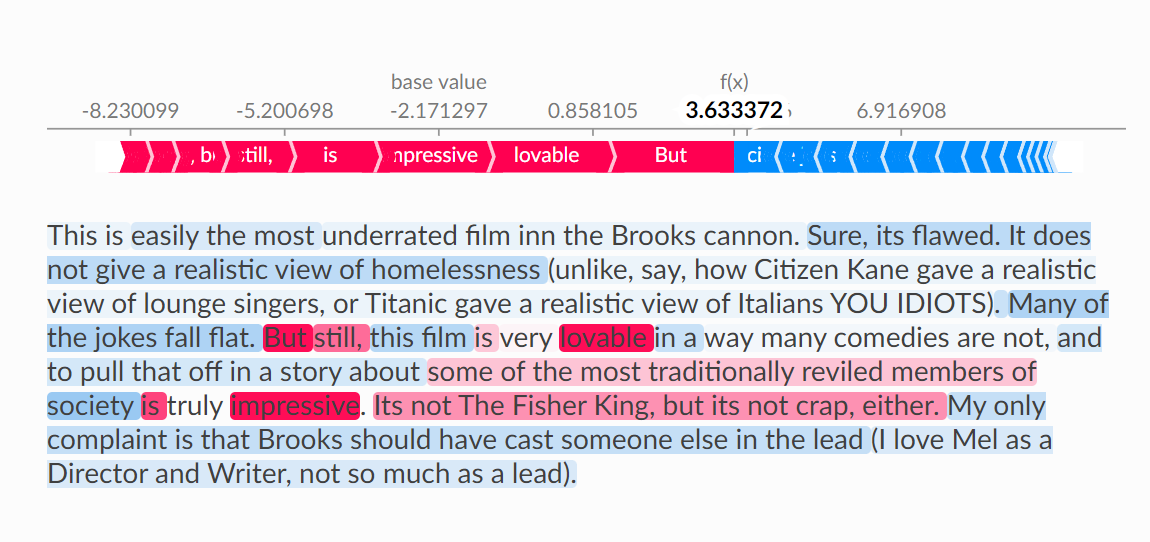
\includegraphics[width=0.8\ancho]{figs/shap_example.png}
    \caption{Ejemplo de visualización \citep{SHAPtextplot}}
    \label{fig:shap-ex}
\end{figure}

El color rojo indica tendencia a la clase positiva y el azul a la clase negativa. A partir del \textit{base value} y $f(x)$ indicados en el eje de la parte superior, podemos conocer cuál es el resultado de la clasificación comparándolos: si $f(x) > \textit{base value}$ la clasificación será positiva, mientras que si $f(x) < \textit{base value}$ será negativa. Por último, podemos ver la contribución de cada token en ambas partes: en la parte superior, el tamaño de los tokens varía según importancia o contribución a la clasificación; en la parte inferior esta relación se representa usando la intensidad de color, mayor intensidad indica mayor importancia.

Partiendo de estas nociones, podemos analizar el `razonamiento'\ de estos modelos utilizando ejemplos de noticias del conjunto de test, mostrando algunos ejemplos representativos.

\subsection{Politifact-Snopes One Evidence}

\begin{figure}[!h]
    \captionsetup[subfigure]{justification=Centering}

    % DistilBERT BASE (CASED / CASED MULTILINGUAL)
    \begin{subfigure}[t]{0.4\textwidth}
        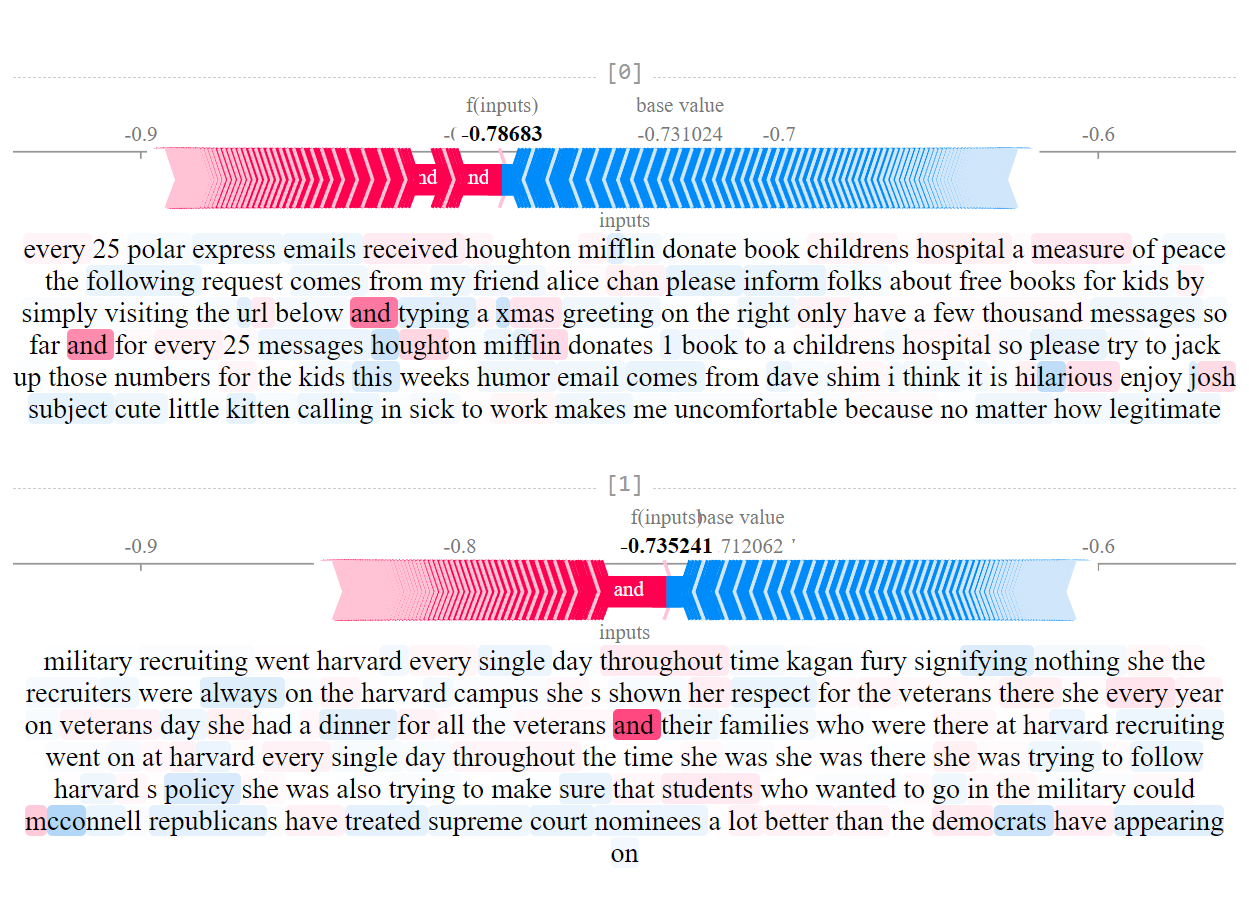
\includegraphics[width=\textwidth]{figs/one_TF/distil-b-c.png}
        \caption{{DistilBERT}\textsubscript{B, C}}
    \end{subfigure}
    \hspace{\fill} % maximize horizontal separation
    \begin{subfigure}[t]{0.4\textwidth}
        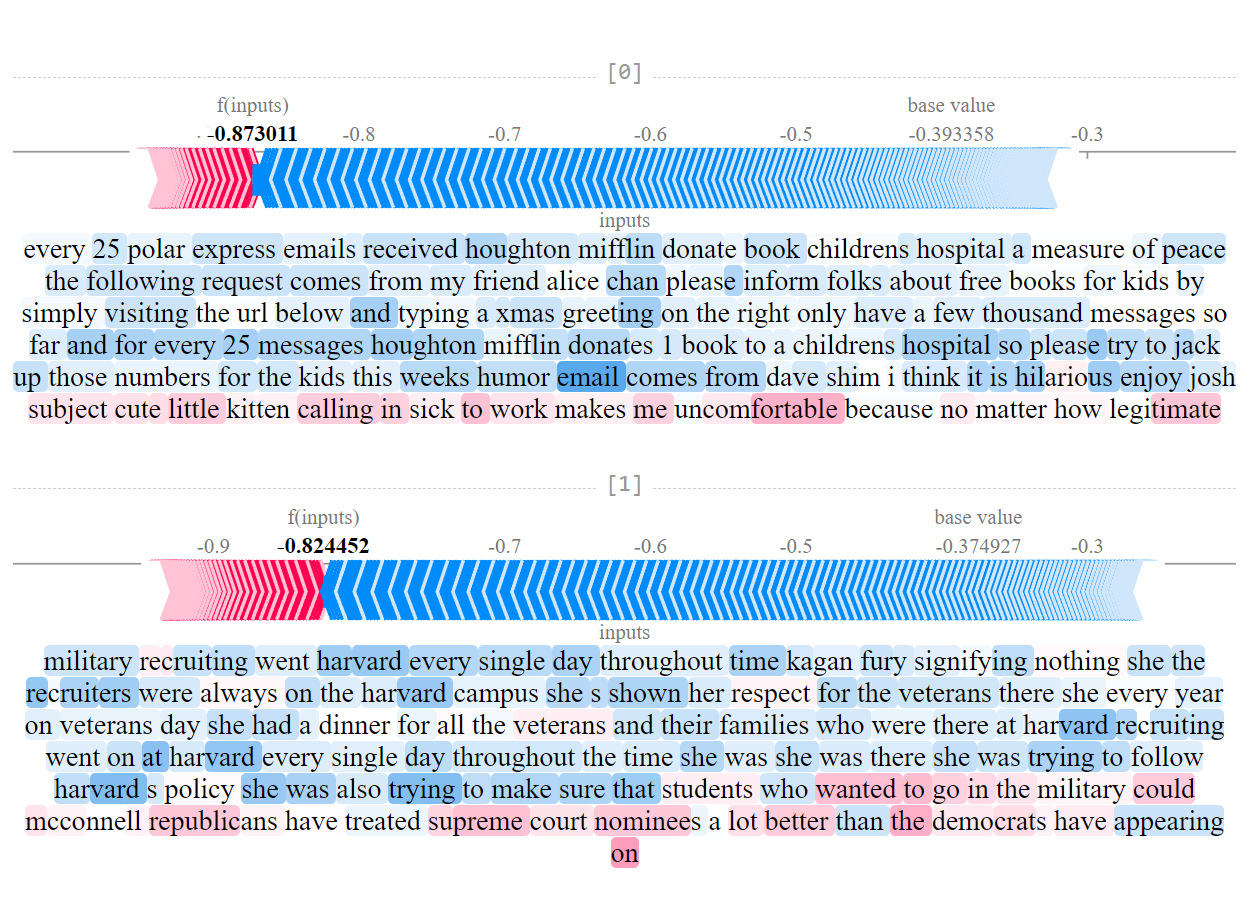
\includegraphics[width=\linewidth]{figs/one_TF/bert-b-ml-c.png}
        \caption{{DistilBERT}\textsubscript{B, C, ML}}
    \end{subfigure}
    
    \caption{Valores Shapley de cada modelo para dos noticias: una verdadera y una falsa del \textit{dataset} {P-S}\textsubscript{One}. Los subíndices utilizados para cada modelo $M$ indican respectivamente $M_{\text{B}}$: BASE; $M_{C}$: CASED; $M_{\text{ML}}$: MULTILINGUAL.}
    \label{fig:shap-ps-one}
\end{figure}

En este caso la primera noticia (superior) es verdadera, mientras que la segunda (inferior) falsa. Observamos que en ambos casos, los dos modelos tienden a la clase negativa en mayor o menor medida. 

Centrándonos en los ejemplos de la figura \hyperref[fig:shap-ps-one]{6.2} vemos que {DistilBERT}\textsubscript{B, C, ML} tiene una distribución de los valores Shapley más uniforme que en {DistilBERT}\textsubscript{B, C}. Parece que {DistilBERT}\textsubscript{B, C, ML} `presta más atención'\ a los \textit{tokens} individuales y menos a los colindantes. Esto nos puede dar la intuición de que este modelo parece `entender'\ el texto en general y por consecuencia, entender el estilo o la estructura sintáctica. 

También podemos hipotetizar que este comportamiento se debe al hecho de que este dataset no tiene ningún signo de puntuación ni capitalización, por lo que en el caso de los modelos CASED no pueden hacer uso de todas estas features para clasificar las noticias.

Analizando el comportamiento de los demás modelos (véase Apéndice \hyperref[fig:shap-ps-one-annex]{A.2.1.}), observamos que esta tendencia es parecida para {BERT}\textsubscript{B, C, ML}; {BERT}\textsubscript{L, U}; {BERT}\textsubscript{L, C}; {RoBERTa}\textsubscript{L} y {DeBERTa}\textsubscript{B}. Por otro lado, también encontramos otros modelos como {BERT}\textsubscript{B, U, ML}; {RoBERTa}\textsubscript{B} y {DeBERTa}\textsubscript{L} que prácticamente no parecen `prestar atención'\ a ningún token del texto. En estos casos los valores de \textit{base value} y $f(x)$ \textit{(logits)} también son muy similares, por lo que pensamos que con estos ejemplos los modelos no son capaces de encontrar las \textit{features} que caracterizan o no una \textit{fake news}.

En conclusión, observamos que algunos de los modelos parecen ser sensibles a estructuras más complejas que el \textit{token} individual, ya que la atención o la importancia de estos \textit{tokens} está más repartida a lo largo de la frase. Aún así, estos resultados no parecen ser concluyentes porque esa atención no está distribuida equitativamente a lo largo de la frase y tampoco el modelo consigue clasificar correctamente estos fragmentos.

\subsection{Politifact-Snopes All Evidences}

\begin{figure}[!h]
    \captionsetup[subfigure]{justification=Centering}
  \captionsetup[subfigure]{justification=Centering}

    % BERT BASE MULTILINGUAL (UNCASED / CASED)
    \begin{subfigure}[t]{0.4\textwidth}
        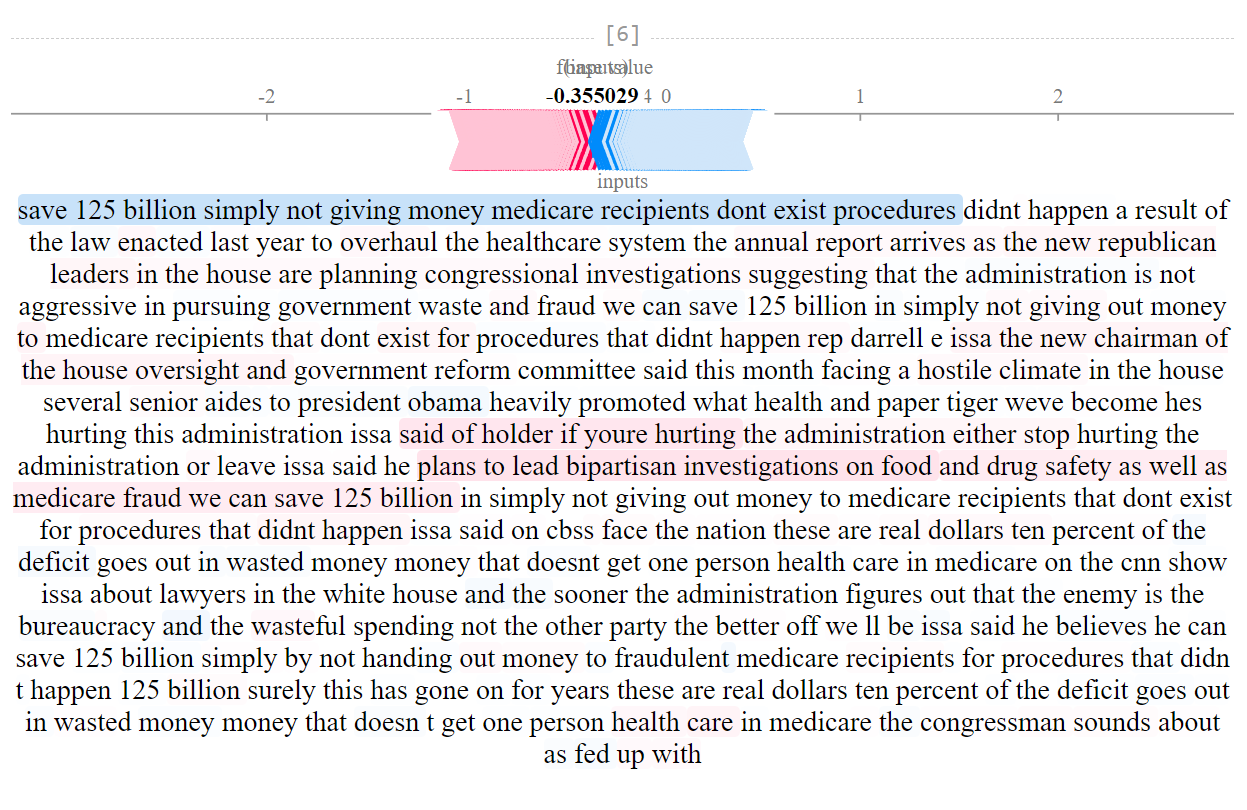
\includegraphics[width=\textwidth]{figs/all_F/bert-b-ml-u.png}
        \caption{{BERT}\textsubscript{B, U, ML}}
    \end{subfigure}
    \hspace{\fill} % maximize horizontal separation
    \begin{subfigure}[t]{0.4\textwidth}
        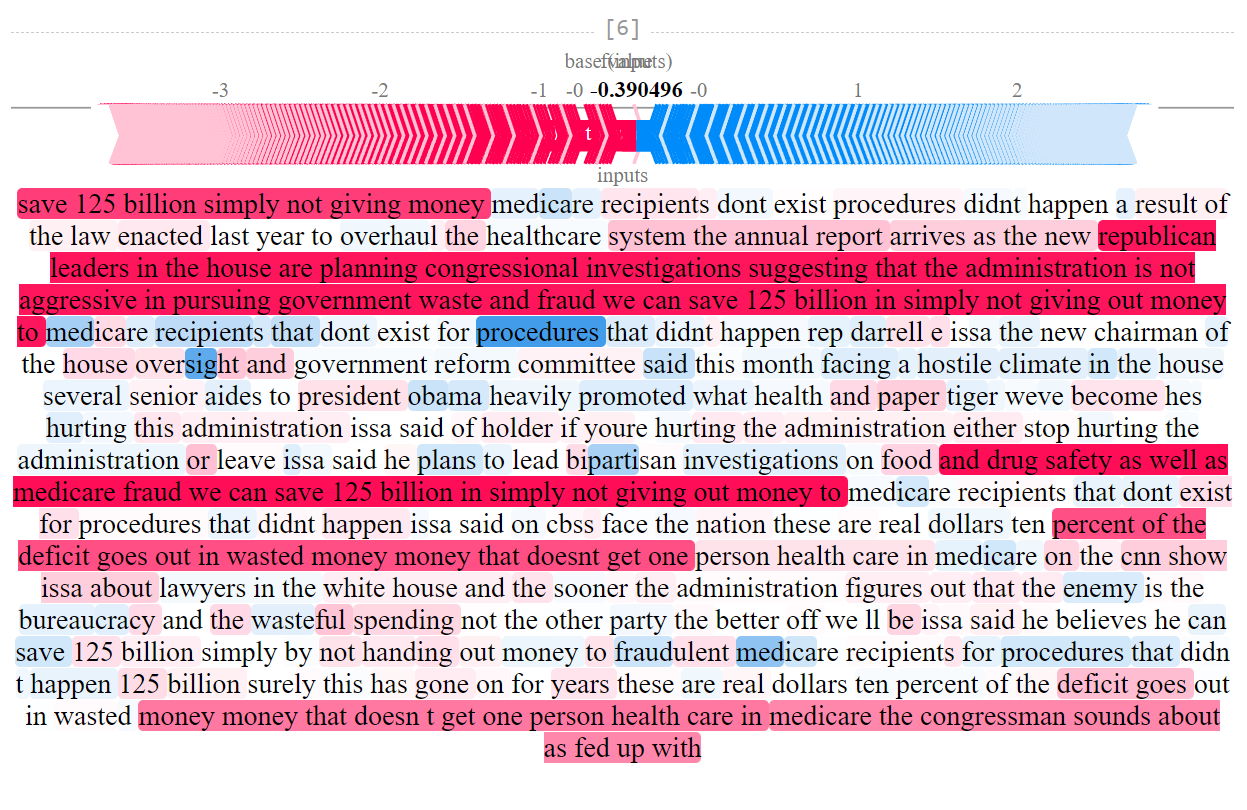
\includegraphics[width=\linewidth]{figs/all_F/bert-b-ml-c.png}
        \caption{{BERT}\textsubscript{B, C, ML}}
    \end{subfigure}  
    
    \caption{Valores Shapley de cada modelo para una noticia falsa del \textit{dataset} {P-S}\textsubscript{All}. Los subíndices utilizados para cada modelo $M$ indican respectivamente $M_{\text{B}}$: BASE; $M_{C}$: CASED; $M_{\text{U}}$: UNCASED; $M_{\text{ML}}$: MULTILINGUAL.}
    \label{fig:shap-ps-all}
\end{figure}

El ejemplo elegido es de una noticia falsa o \textit{fake news}, en la figura \hyperref[fig:shap-ps-all]{6.3} notamos que {BERT}\textsubscript{B, C, ML} parece `prestar atención' a estructuras más complejas que en el caso anterior. Leyendo las partes subrayadas con más intensidad nos da a entender que el modelo está `entendiendo' frases. Concretamente, estas frases son ``save 125 billion simply not giving money'', ``(investigations on food) and drug safety as well as medicare fraud we can save 125 billion in simply not giving out money to (medicare recipients that dont exist'', ``(ten) percent of the deficit goes out in wasted money [...]''. Estas frases son muy concisas, característica clave de las \textit{fake news}.

Por otro lado, {BERT}\textsubscript{B, U, ML} presta muy poca atención en comparación con el ejemplo anterior, aunque de la poca atención que presta, parece hacerlo también en frases y no \textit{tokens} individuales. Aún así, en ambos casos el resultado de la clasificación no parece influir, ya que los \textit{base value} y $f(x)$ son muy parecidos.

Los demás modelos (véase Apéndice \hyperref[fig:shap-ps-all-annex]{A.2.2.}) parecen seguir la tendencia de {BERT}\textsubscript{B, C, ML}; resaltando frases concretas, estos son concretamente: {BERT}\textsubscript{B, U}; {DistilBERT}\textsubscript{B, C}; {DistilBERT}\textsubscript{B, C, ML}; {RoBERTa}\textsubscript{B} y {DeBERTa}\textsubscript{L}. Los \textit{logits} obtenidos, reflejados en el valor $f(x)$, generalmente son mayores a los \textit{base values}, por lo que las clasificaciones realizadas son correctas y con un cierto grado de confianza.

El resto, sigue el comportamiento de {BERT}\textsubscript{B, U, ML}; con poca o nula atención a frases. Los \textit{logits} también son muy similares a los \textit{base values}, por lo que no parece haber mucha confianza en la predicción.

\subsection{News}

\begin{figure}[!h]
    \captionsetup[subfigure]{justification=Centering}

    % RoBERTa (BASE / LARGE)
    \begin{subfigure}[t]{0.4\textwidth}
        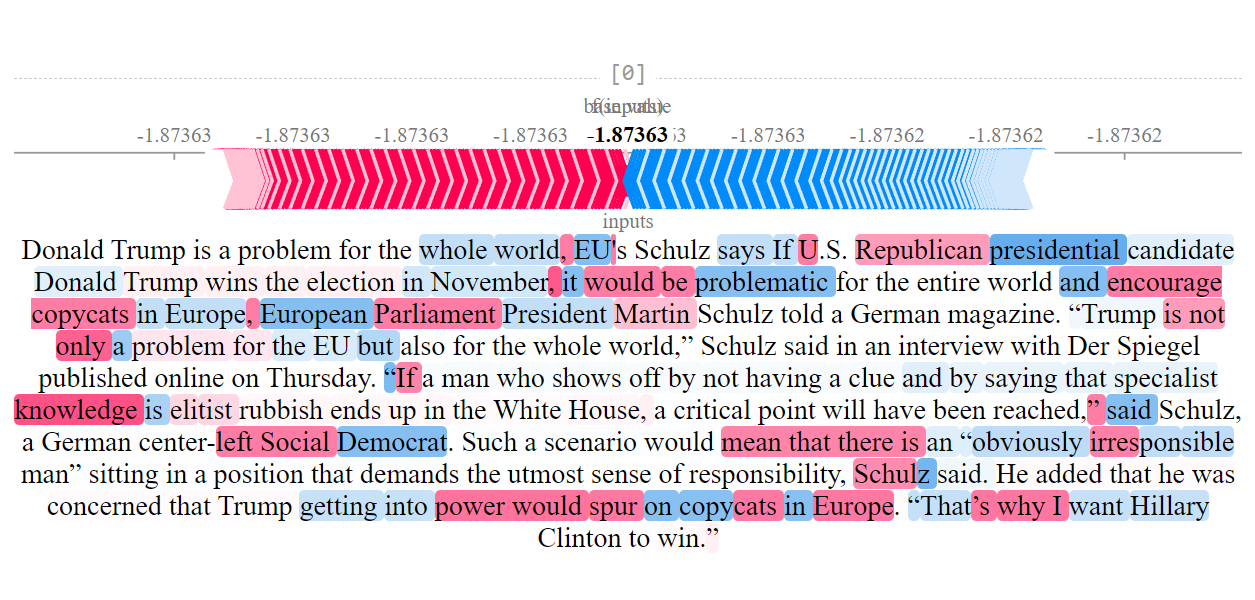
\includegraphics[width=\textwidth]{figs/news_T/roberta-b.png}
        \caption{{RoBERTa}\textsubscript{B}}
    \end{subfigure}
    \hspace{\fill} % maximize horizontal separation
    \begin{subfigure}[t]{0.4\textwidth}
        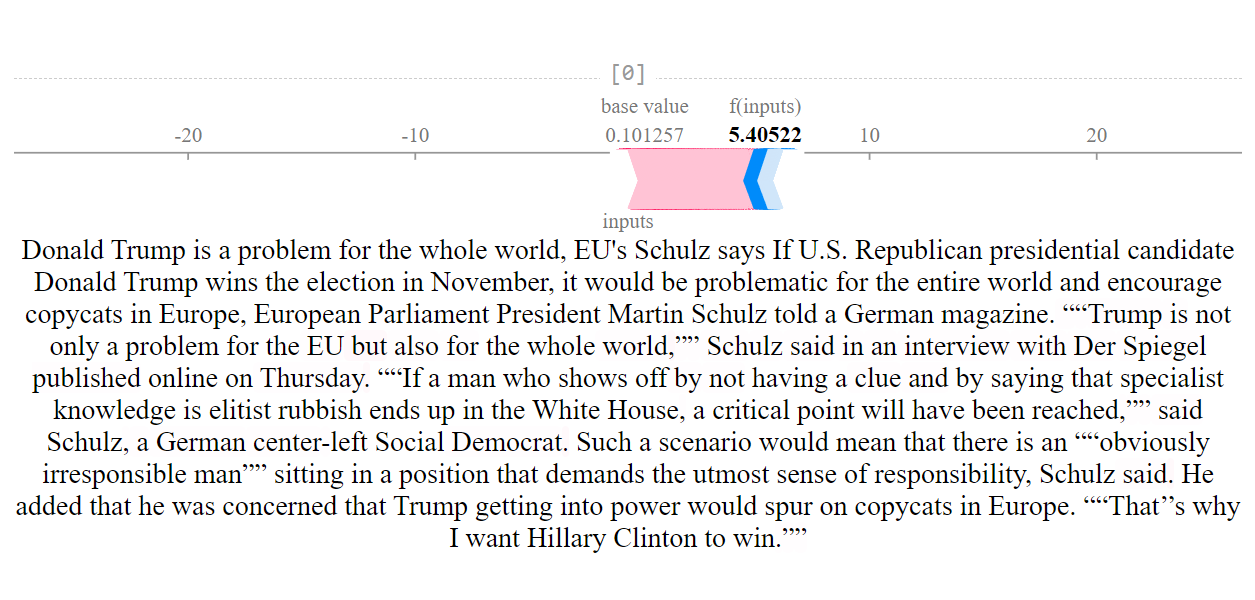
\includegraphics[width=\linewidth]{figs/news_T/roberta-l.png}
        \caption{{RoBERTa}\textsubscript{L}}
    \end{subfigure}
    
    \caption{Valores Shapley para una noticia verdadera del \textit{dataset} News. Los subíndices utilizados para cada modelo $M$ indican respectivamente $M_{\text{B}}$: BASE; $M_{\text{L}}$: LARGE.}
    
\end{figure}

Teniendo en cuenta que la noticia es verdadera, podemos observar que el peso de los \textit{tokens} para {RoBERTa}\textsubscript{B} son ínfimos en comparación con {RoBERTa}\textsubscript{L}. Este último modelo no parece resaltar ningún token como relevante para hacer la predicción. 

Este ejemplo no es aislado, esta tendencia es común a los siguientes modelos: {BERT}\textsubscript{B, U}; {BERT}\textsubscript{B, C, ML}; {BERT}\textsubscript{L, C}; {DistilBERT}\textsubscript{B, C}; {DistilBERT}\textsubscript{B, C, ML}; {RoBERTa}\textsubscript{L}; {DeBERTa}\textsubscript{B} y {DeBERTa}\textsubscript{L}. Solamente cuatro modelos de doce parecen al menos `razonar'\ y prestan atención a tokens concretos. Aún así, este `razonamiento'\ que tienen los otros modelos no parece tener mucho sentido tampoco, ya que suelen prestar atención a tokens sueltos y no a estructuras sintácticas concretas, cosa que no esperábamos.

Estos modelos parecen funcionar peor con este dataset que en los casos anteriores: la atención está muy distribuida de forma muy poco uniforme, los \textit{logits} tienen valores muy bajos en relación a los \textit{base values} o son extremadamente mayores (esto sucede en la mayoría de modelos que `no prestan atención'\ a ninguno de los \textit{tokens} en el texto.

\section{Evaluación}
\label{sec:eval}

Habiendo analizado los resultados en la sección \hyperref[sec:results]{6.1}, podemos deducir que los modelos entrenados no parecen funcionar correctamente para detectar \textit{fake-news} gracias a sus características estilísticas. Aún así, viendo las métricas de \textit{specificity}, creemos que mediante esta metodología hemos creado un sistema capaz de detectar las \textit{features} que hacen que una noticia sea verdadera, concretamente los modelos LARGE, {DistilBERT}\textsubscript{B, C, ML}; {BERT}\textsubscript{B, C} y {DeBERTa}\textsubscript{B} son los que ofrecen mejores métricas para los \textit{datasets} de PolitiFact-Snopes, siendo los modelos LARGE los más consistentes en todos los \textit{datasets}.

En la sección \hyperref[sec:shap]{6.2} hemos intentando entender cuál es el funcionamiento o razonamiento interno detrás de estos modelos a la hora de clasificar. Utilizando los valores Shapley, hemos modelizado la atención de estos modelos y mediante ellos determinar qué palabras o frases son las más importantes en la clasificación.

En general, los resultados no eran los esperados, ya que las métricas obtenidas en la sección \hyperref[sec:results]{6.1} nos daban una visión más optimista del rendimiento de estos modelos. El \textit{dataset} con el que hemos obtenido el mejor rendimiento ha sido {P-S}\textsubscript{All}, el siguiente {P-S}\textsubscript{One} y el peor News.

Es por ello que creemos que es necesario investigar en profundidad otros factores resaltados en la sección \hyperref[sec:results]{6.1}, como la pérdida de rendimiento general de los modelos BASE al añadir más evidencias o al entrenar con el \textit{dataset} News, o en la sección \hyperref[sec:shap]{6.2}, como los mecanismos de atención de estos modelos y el pobre funcionamiento con el \textit{dataset} News.